
\section{Ising Nonuniversality}
The braiding matrices for Ising anyons are given by Eqs. $10.10$ and $10.11$. Demonstrate that any multiplication of these matrices, and their inverses will only produce a finite number of possible results. Thus conclude that Ising anyons are not universal for quantum computation. Hint: write the braiding matrices as $\mathrm{e}^{\mathrm{i} \alpha } U_{i}$ where $U_{i}$ is unitary with unit determinant, i.e., is an element of $SU(2)$. Then note that any $SU(2)$ matrix can be thought of as a rotation $\exp (\mathrm{i}\hat{n} \cdot \boldsymbol{\sigma } \theta /2)$ where here $\theta $ is an angle of rotation $\hat{n}$ is the axis of rotation and $\boldsymbol{\sigma }$ is the vector of Pauli spin matrices.

\paragraph{Answer}
We are given that
\begin{equation*}
\begin{aligned}
\hat{\sigma }_{1} & =\mathrm{e}^{-\mathrm{i} \pi /8}\begin{pmatrix}
1 & 0\\
0 & \mathrm{i}
\end{pmatrix} =\mathrm{e}^{\mathrm{i} \pi /8}\begin{pmatrix}
\mathrm{e}^{-\mathrm{i} \pi /4} & 0\\
0 & \mathrm{e}^{\mathrm{i} \pi /4}
\end{pmatrix} \equiv \mathrm{e}^{\mathrm{i} \pi /8} U_{1} ,\\
\hat{\sigma }_{2} & =\frac{\mathrm{e}^{\mathrm{i} \pi /8}}{\sqrt{2}}\begin{pmatrix}
1 & -\mathrm{i}\\
-\mathrm{i} & 1
\end{pmatrix} =\mathrm{e}^{\mathrm{i} \pi /8}\begin{pmatrix}
1/\sqrt{2} & -\mathrm{i} /\sqrt{2}\\
-\mathrm{i} /\sqrt{2} & 1/\sqrt{2}
\end{pmatrix} \equiv \mathrm{e}^{\mathrm{i} \pi /8} U_{2} .
\end{aligned}
\end{equation*}
Here $\det U_{1} =\det U_{2} =1$. Now we can write $U_{1}$,$U_{2}$ in the form of generators of $SU( 2)$:
\begin{equation*}
U_{1} =\begin{pmatrix}
\mathrm{e}^{-\mathrm{i} \pi /4} & 0\\
0 & \mathrm{e}^{\mathrm{i} \pi /4}
\end{pmatrix} =\exp( -\mathrm{i} \pi \sigma _{z} /4) ,
\end{equation*}
and
\begin{equation*}
U_{2} =\begin{pmatrix}
\cos( -\pi /4) & \mathrm{i}\sin( -\pi /4)\\
\mathrm{i}\sin( -\pi /4) & \cos( -\pi /4)
\end{pmatrix} =\exp( -\mathrm{i} \pi \sigma _{x} /4) .
\end{equation*}
Now we try to prove the group generated by $U_{1} ,U_{2}$ is finite. We can see
\begin{equation*}
U_{1} U_{2} U_{1}^{-1} =U_{3} \equiv \exp( -\mathrm{i} \pi \sigma _{y} /4) ,
\end{equation*}
This is to say:
\begin{equation*}
U_{1} U_{2} =U_{3} U_{1} .
\end{equation*}
Now any element generated by $U_{1} ,U_{2}$ can be written in the form
\begin{equation*}
U_{2}^{m} U_{3}^{n} U_{1}^{k} ,
\end{equation*}
where $0\leq m,n,k\leq 8$. For example:
\begin{equation*}
U_{1} U_{2} U_{1} =U_{3} U_{1}^{2} ,U_{2}^{2} U_{1} U_{2} =U_{2}^{2} U_{3} U_{1} .
\end{equation*}
By listing all its elements, we can find it is a finite group of order 48. It has a normal subgroup\cite{GAP4}
\begin{equation*}
\left< \frac{1}{2}\begin{pmatrix}
-1+\mathrm{i} & -1-\mathrm{i}\\
1-\mathrm{i} & -1-\mathrm{i}
\end{pmatrix} ,\begin{pmatrix}
0 & -1\\
1 & 0
\end{pmatrix} ,\begin{pmatrix}
-\mathrm{i} & 0\\
0 & \mathrm{i}
\end{pmatrix} ,\begin{pmatrix}
-1 & 0\\
0 & -1
\end{pmatrix}\right> \cong SL( 2,3) ,
\end{equation*}
and
\begin{equation*}
\left< \begin{pmatrix}
0 & -1\\
1 & 0
\end{pmatrix} ,\begin{pmatrix}
-\mathrm{i} & 0\\
0 & \mathrm{i}
\end{pmatrix} ,\begin{pmatrix}
-1 & 0\\
0 & -1
\end{pmatrix}\right> \cong \mathbb{Q}_{8} ,
\end{equation*}
and
\begin{equation*}
\left< \begin{pmatrix}
-1 & 0\\
0 & -1
\end{pmatrix}\right> \cong \mathbb{Z}_{2} .
\end{equation*}
Actually, the group generated by $\langle U_{1} ,U_{2} \rangle $ is a generalization of the famous \textbf{Von Dyck group}\cite{stoytchev2020class}. The general Von Dyck group is defined by the presentation:
\begin{equation*}
D( l,m,n) =\langle x,y|x^{l} =y^{m} =(xy )^{n} =1\rangle .
\end{equation*}
This kind of group is \textbf{finite if and only if}
\begin{equation*}
\frac{1}{l} +\frac{1}{m} +\frac{1}{n}  >1.
\end{equation*}
If we try to construct:
\begin{equation*}
x\equiv U_{1} U_{2} U_{1} ,\quad y\equiv U_{1} U_{2} ,
\end{equation*}
then we will find easily:
\begin{equation*}
x^{2} =y^{3} =( xy)^{4} =-\mathds{1}_{2} .
\end{equation*}
The case $D( 2,3,4)$ is just $S_{4}$, and our group $G\equiv \langle U_{1} ,U_{2} \rangle $ is actually the group extension of $D( 2,3,4)$. We can construct the short exact sequence
\begin{equation*}
\mathds{1}\rightarrow \mathbb{Z}_{2}\rightarrow G\rightarrow S_{4}\rightarrow \mathds{1} ,
\end{equation*}
which is a non-split exact sequence. As the presentation above shows, it can be considered as ``double copy'' of $D( 2,3,4) \cong S_{4}$. 

\section{Brute Force Search}
Given the braid matrices for Fibonacci anyons in Eq. 10.6 and 10.7, write a computer program for brute-force searching braids up to length 10.



Ignoring the noncomputational state $|N\rangle $, and ignoring the overall phase as usual, determine the closest approximation to the Hadamard gate
\begin{equation*}
H=\frac{1}{\sqrt{2}}\begin{pmatrix}
1 & 1\\
1 & -1
\end{pmatrix}
\end{equation*}
Partial Answer: A braid of length 10 exists with phase-invariant distance to target dist $\approx 0.084$

\paragraph{Answer}
After brute force search, the closest braiding is given by
\begin{equation*}
\begin{aligned}
U_{1} =\hat{\sigma }_{2}^{-1}\hat{\sigma }_{1}^{-1}\hat{\sigma }_{2}^{-2}\hat{\sigma }_{1}^{-1}\hat{\sigma }_{2}^{-2}\hat{\sigma }_{1}^{-1}\hat{\sigma }_{2}^{-1} & =\begin{pmatrix}
0.190983\ +0.587785\mathrm{i} & 0.242934\ +0.747674\mathrm{i}\\
0.242934\ +0.747674\mathrm{i} & -0.190983-0.587785\mathrm{i}
\end{pmatrix} ,\\
U_{2} =\hat{\sigma }_{2}^{-1}\hat{\sigma }_{2}^{-3}\hat{\sigma }_{1}^{-1}\hat{\sigma }_{2}^{-1}\hat{\sigma }_{1}^{3} & =\begin{pmatrix}
0.190983\ +0.587785\mathrm{i} & 0.242934\ +0.747674\mathrm{i}\\
0.242934\ +0.747674\mathrm{i} & -0.190983-0.587785\mathrm{i}
\end{pmatrix} .
\end{aligned}
\end{equation*}
Their distances are given by:
\begin{equation*}
\operatorname{dist}( H,U_{1}) =\operatorname{dist}( H,U_{2}) \approx 0.08421.
\end{equation*}
The mathematica code is given in the attached file. 

\section{Scaling of Kitaev-Solovay Algorithm}
Given the discussion just above Eq. 11.8, prove Eqs. 11.8 and 11.9.

\paragraph{Answer}
Suppose we want to get a target gate $U_{\text{target}}^{( 0)}$. Using brute-force search, we can get $U_{\text{approx}}^{( 0)}$ in $t_{0}$ steps within the distance $\epsilon _{0}$. Then we define
\begin{equation*}
U_{\text{target}}^{( 1)} \equiv [U_{\text{approx}}^{( 0)} ]^{-1} U_{\text{target}}^{( 0)} ,
\end{equation*}
which close to identity within distance $\epsilon _{0}$. With decomposition
\begin{equation*}
U_{\text{target}}^{( 1)} =VWV^{-1} W^{-1} ,
\end{equation*}
and $W$ and $V$ being unitary operations close to the identity within $\epsilon _{0}^{1/2}$, we can approximate $U_{\text{target }}^{(0)}$ with accuracy $\epsilon _{0}^{3/2}$. Now the total length is $5t_{0}$, and by $n$ iteration, the accuracy is
\begin{equation*}
\epsilon =\epsilon _{0}^{( 2/3)^{n}} ,
\end{equation*}
with length 
\begin{equation*}
t=5^{n} t_{0} .
\end{equation*}
So for large $n$:
\begin{equation*}
\ln [\log (1/\epsilon )]/\ln (3/2)\sim \ln (t)/\ln (5),
\end{equation*}
which means
\begin{equation*}
t\sim \mathcal{O}\left(\log (1/\epsilon )^{\ln (5)/\ln (3/2)}\right) .
\end{equation*}
For classical computation, the time consumed by $n$ iteration is
\begin{equation*}
T=3^{n} T_{0} ,
\end{equation*}
which means
\begin{equation*}
T\sim \mathcal{O}\left(\log (1/\epsilon )^{\ln (3)/\ln (3/2)}\right) .
\end{equation*}

\section{About the Injection Weave}
One might wonder why we choose to work with an injection weave in Fig. $11.11$ which moves the red strand from the far right at the bottom all the way to the far left on the top. Show that for three Fibonacci anyons, there does not exist any injection weave that moves the (red) strand from the far right on the bottom to the middle on the top, even up to an overall phase. I.e., show that no weave exists starting on the bottom far left ending in the middle on the top whose effect on the three dimensional Hilbert space is $\mathrm{e}^{\mathrm{i} \phi }\mathds{1}_{3\times 3}$ for any phase $\phi $.

\paragraph{Answer}
Suppose such operation exists, i.e. exits any injection weave that moves the red strand from the far right on the bottom to the middle on the top, which equals to $U=\mathrm{e}^{\mathrm{i} \phi }\mathds{1}_{3}$. Assume $\hat{\sigma }_{1}$ appears $m$ times in the $U$($\hat{\sigma }_{1}^{-1}$ contributes $-1$ to $m$) and $\hat{\sigma }_{2}$ appears $n$ times in the sequence. Note that for $|N \rangle $, the braiding matrix is block-diagonal, which means
\begin{equation*}
\exp( 3( m+n) \pi \mathrm{i} /5) =\exp(\mathrm{i} \phi ) ,
\end{equation*}
i.e.
\begin{equation*}
\phi =3( m+n) \pi /5+2k\pi .
\end{equation*}
We can take det of eq $U=\mathrm{e}^{\mathrm{i} \phi }\mathds{1}_{3}$, using $\det\hat{\hat{\sigma }}_{1} =\det\hat{\hat{\sigma }}_{2} =\mathrm{e}^{2\pi \mathrm{i} /5}$, we will have
\begin{equation*}
\exp( 2( m+n) \pi \mathrm{i} /5) =\exp( 3\mathrm{i} \phi ) ,
\end{equation*}
i.e.
\begin{equation*}
3\phi =2( m+n) \pi \mathrm{i} /5+2k'\pi .
\end{equation*}
Combine two equations:
\begin{equation*}
m+n=\frac{10}{7}( k'-3k) .
\end{equation*}
However, note that if $m+n$ is an integer, it must be even according to this formula, but our operation is an odd permutation, which means $m+n$ should be odd, contradicts. So such injection weave doesn't exist. 

\section{Universal Weaving and the Injection Weave}
Consider injection weaves as described in Fig. 11.11. Let us assume that we can construct an injection weave of arbitrary precision. Given such an (approximately) perfect injection weave show that for any number of anyons $N >3$, a weave can be constructed that performs the same unitary operation on the Hilbert space as any given braid. A more general mathematical proof of the universality of weaving is also given in Simon et al. [2006].

\paragraph{Answer}
Suppose there are $N$ anyons, as the Fig. \ref{fig:NAnyonWithNumber} shows.
\begin{figure}[h!]
\centering
\tikzset{every picture/.style={line width=0.75pt}} %set default line width to 0.75pt        

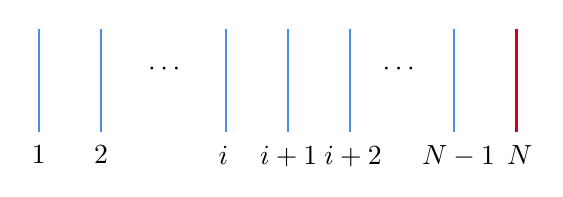
\begin{tikzpicture}[x=0.75pt,y=0.75pt,yscale=-1,xscale=1]
%uncomment if require: \path (0,86); %set diagram left start at 0, and has height of 86

%Straight Lines [id:da9281561089862298] 
\draw [color={rgb, 255:red, 74; green, 144; blue, 226 }  ,draw opacity=1 ]   (206,9) -- (206,59) ;
%Straight Lines [id:da8669553440202185] 
\draw [color={rgb, 255:red, 74; green, 144; blue, 226 }  ,draw opacity=1 ]   (236,9) -- (236,59) ;
%Straight Lines [id:da2623692890994038] 
\draw [color={rgb, 255:red, 74; green, 144; blue, 226 }  ,draw opacity=1 ]   (356,9) -- (356,59) ;
%Straight Lines [id:da9143494559374035] 
\draw [color={rgb, 255:red, 74; green, 144; blue, 226 }  ,draw opacity=1 ]   (296,9) -- (296,59) ;
%Straight Lines [id:da7859416817573242] 
\draw [color={rgb, 255:red, 74; green, 144; blue, 226 }  ,draw opacity=1 ]   (326,9) -- (326,59) ;
%Straight Lines [id:da10249537208282766] 
\draw [color={rgb, 255:red, 208; green, 2; blue, 27 }  ,draw opacity=1 ]   (436,9) -- (436,59) ;
%Straight Lines [id:da9994723584700849] 
\draw [color={rgb, 255:red, 74; green, 144; blue, 226 }  ,draw opacity=1 ]   (406,9) -- (406,59) ;

% Text Node
\draw (257,24) node [anchor=north west][inner sep=0.75pt]    {$\cdots $};
% Text Node
\draw (370,24) node [anchor=north west][inner sep=0.75pt]    {$\cdots $};
% Text Node
\draw (201,64) node [anchor=north west][inner sep=0.75pt]    {$1$};
% Text Node
\draw (231,64) node [anchor=north west][inner sep=0.75pt]    {$2$};
% Text Node
\draw (291,64) node [anchor=north west][inner sep=0.75pt]    {$i$};
% Text Node
\draw (311,64) node [anchor=north west][inner sep=0.75pt]    {$i+1$};
% Text Node
\draw (342,64) node [anchor=north west][inner sep=0.75pt]    {$i+2$};
% Text Node
\draw (389,64) node [anchor=north west][inner sep=0.75pt]    {$N-1$};
% Text Node
\draw (430,64) node [anchor=north west][inner sep=0.75pt]    {$N$};
\end{tikzpicture}
\caption{$N$ anyons with number $1$ to $N$.}
\label{fig:NAnyonWithNumber}
\end{figure}

Any braiding can be generated by $\hat{\sigma }_{i}$, $1\leq i\leq N-1$. Suppose we want to perform $\hat{\sigma }_{i}$, we can view strand $i+2$ to $N-1$ as a single strand $c$ according to locality. Then we perform the injection weave between $i+1,c$ and $N$, as the Fig.\ref{fig:WeaveRealizationSigma} shows. After that, we do $\hat{\sigma }_{i}$ between $i$ and the red line. Finally, we view strand $i+2$(blue) to $N$(green) as a single strand $c'$ and perform the inverse injection. This is a weave and has the effect of $\hat{\sigma }_{i}$ purely. 

\begin{figure}[h!]
\centering
\tikzset{every picture/.style={line width=0.75pt}} %set default line width to 0.75pt        

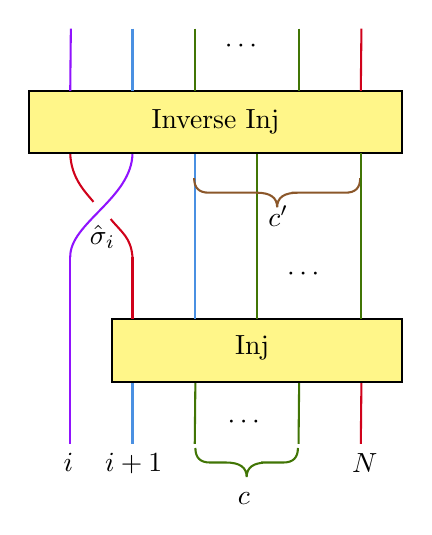
\begin{tikzpicture}[x=0.75pt,y=0.75pt,yscale=-1,xscale=1]
%uncomment if require: \path (0,241); %set diagram left start at 0, and has height of 241

%Straight Lines [id:da4652666292395473] 
\draw [color={rgb, 255:red, 65; green, 117; blue, 5 }  ,draw opacity=1 ]   (320.3,173) -- (320,203) ;
%Straight Lines [id:da5483996794596906] 
\draw [color={rgb, 255:red, 144; green, 19; blue, 254 }  ,draw opacity=1 ]   (260,113) -- (260,203) ;
%Straight Lines [id:da4508386291891626] 
\draw [color={rgb, 255:red, 74; green, 144; blue, 226 }  ,draw opacity=1 ]   (290,173) -- (290,203) ;
%Straight Lines [id:da8256137577460634] 
\draw [color={rgb, 255:red, 208; green, 2; blue, 27 }  ,draw opacity=1 ]   (400.3,173) -- (400,203) ;
%Straight Lines [id:da2421069879995652] 
\draw [color={rgb, 255:red, 65; green, 117; blue, 5 }  ,draw opacity=1 ]   (370.3,173) -- (370,203) ;
%Shape: Brace [id:dp2745768049942996] 
\draw  [color={rgb, 255:red, 65; green, 117; blue, 5 }  ,draw opacity=1 ] (320.3,205) .. controls (320.3,209.67) and (322.63,212) .. (327.3,212) -- (335,212) .. controls (341.67,212) and (345,214.33) .. (345,219) .. controls (345,214.33) and (348.33,212) .. (355,212)(352,212) -- (362.7,212) .. controls (367.37,212) and (369.7,209.67) .. (369.7,205) ;
%Shape: Rectangle [id:dp47335305318361875] 
\draw  [fill={rgb, 255:red, 255; green, 246; blue, 137 }  ,fill opacity=1 ] (280,143) -- (420,143) -- (420,173) -- (280,173) -- cycle ;
%Straight Lines [id:da21833313269743537] 
\draw [color={rgb, 255:red, 208; green, 2; blue, 27 }  ,draw opacity=1 ]   (290,113) -- (290,143) ;
%Straight Lines [id:da6139776773522196] 
\draw [color={rgb, 255:red, 74; green, 144; blue, 226 }  ,draw opacity=1 ]   (320,63) -- (320,143) ;
%Straight Lines [id:da007808682261698063] 
\draw [color={rgb, 255:red, 65; green, 117; blue, 5 }  ,draw opacity=1 ]   (350,63) -- (350,143) ;
%Curve Lines [id:da8890702546948639] 
\draw [color={rgb, 255:red, 144; green, 19; blue, 254 }  ,draw opacity=1 ]   (260,113) .. controls (259.7,96.67) and (289.7,84.67) .. (290,63) ;
%Curve Lines [id:da7778590733916251] 
\draw [color={rgb, 255:red, 208; green, 2; blue, 27 }  ,draw opacity=1 ]   (290,113) .. controls (289.19,103.56) and (284.91,101.27) .. (279.48,94.7) ;
%Curve Lines [id:da18463407475936755] 
\draw [color={rgb, 255:red, 208; green, 2; blue, 27 }  ,draw opacity=1 ]   (271.19,86.42) .. controls (267.76,82.14) and (260.34,75.28) .. (260,63) ;
%Shape: Rectangle [id:dp43549331778607203] 
\draw  [fill={rgb, 255:red, 255; green, 246; blue, 137 }  ,fill opacity=1 ] (240,33) -- (420,33) -- (420,63) -- (240,63) -- cycle ;
%Shape: Brace [id:dp571189639130353] 
\draw  [color={rgb, 255:red, 139; green, 87; blue, 42 }  ,draw opacity=1 ] (319.7,75) .. controls (319.7,79.67) and (322.03,82) .. (326.7,82) -- (349.7,82) .. controls (356.37,82) and (359.7,84.33) .. (359.7,89) .. controls (359.7,84.33) and (363.03,82) .. (369.7,82)(366.7,82) -- (392.7,82) .. controls (397.37,82) and (399.7,79.67) .. (399.7,75) ;
%Straight Lines [id:da5231855253626385] 
\draw [color={rgb, 255:red, 65; green, 117; blue, 5 }  ,draw opacity=1 ]   (400,63) -- (400,143) ;
%Straight Lines [id:da040245996635934755] 
\draw [color={rgb, 255:red, 208; green, 2; blue, 27 }  ,draw opacity=1 ]   (400.3,3) -- (400,33) ;
%Straight Lines [id:da21933191775852423] 
\draw [color={rgb, 255:red, 144; green, 19; blue, 254 }  ,draw opacity=1 ]   (260.3,3) -- (260,33) ;
%Straight Lines [id:da8795001694539943] 
\draw [color={rgb, 255:red, 65; green, 117; blue, 5 }  ,draw opacity=1 ]   (320,3) -- (320,33) ;
%Straight Lines [id:da8636160398664288] 
\draw [color={rgb, 255:red, 65; green, 117; blue, 5 }  ,draw opacity=1 ]   (370,3) -- (370,33) ;
%Straight Lines [id:da496856060202457] 
\draw [color={rgb, 255:red, 74; green, 144; blue, 226 }  ,draw opacity=1 ]   (290,3) -- (290,33) ;

% Text Node
\draw (334.3,188) node [anchor=north west][inner sep=0.75pt]    {$\cdots $};
% Text Node
\draw (255.3,206) node [anchor=north west][inner sep=0.75pt]    {$i$};
% Text Node
\draw (275.3,206) node [anchor=north west][inner sep=0.75pt]    {$i+1$};
% Text Node
\draw (394.3,206) node [anchor=north west][inner sep=0.75pt]    {$N$};
% Text Node
\draw (339.3,225) node [anchor=north west][inner sep=0.75pt]    {$c$};
% Text Node
\draw (347.65,156.83) node   [align=left] {Inj};
% Text Node
\draw (330,48) node   [align=left] {Inverse Inj};
% Text Node
\draw (354,87) node [anchor=north west][inner sep=0.75pt]    {$c'$};
% Text Node
\draw (333,7) node [anchor=north west][inner sep=0.75pt]    {$\cdots $};
% Text Node
\draw (363,117) node [anchor=north west][inner sep=0.75pt]    {$\cdots $};
% Text Node
\draw (268,96) node [anchor=north west][inner sep=0.75pt]    {$\hat{\sigma }_{i}$};
\end{tikzpicture}
\caption{The method to realize $\hat{\sigma }_{i}$, where $1\leq i< N-1$.}
\label{fig:WeaveRealizationSigma}
\end{figure}

For $i< N-1$, this scheme applies to every $i$, however, when $i=N-1$, things gets different, we should use the scheme as the Fig.\ref{fig:WeaveRealizationSigmaN-1} shows. 
\begin{figure}[h!]
\centering
\tikzset{every picture/.style={line width=0.75pt}} %set default line width to 0.75pt        

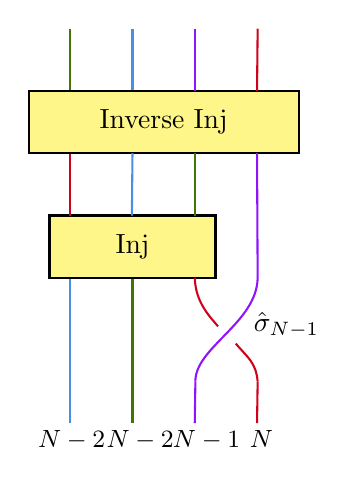
\begin{tikzpicture}[x=0.75pt,y=0.75pt,yscale=-1,xscale=1]
%uncomment if require: \path (0,213); %set diagram left start at 0, and has height of 213

%Straight Lines [id:da6049914954814148] 
\draw [color={rgb, 255:red, 65; green, 117; blue, 5 }  ,draw opacity=1 ]   (310,124) -- (310,194) ;
%Straight Lines [id:da19666615893332962] 
\draw [color={rgb, 255:red, 74; green, 144; blue, 226 }  ,draw opacity=1 ]   (280,124) -- (280,194) ;
%Straight Lines [id:da590664430393607] 
\draw [color={rgb, 255:red, 208; green, 2; blue, 27 }  ,draw opacity=1 ]   (370.3,174) -- (370,194) ;
%Straight Lines [id:da3819935045457825] 
\draw [color={rgb, 255:red, 144; green, 19; blue, 254 }  ,draw opacity=1 ]   (340.3,174) -- (340,194) ;
%Shape: Rectangle [id:dp22673306926244163] 
\draw  [fill={rgb, 255:red, 255; green, 246; blue, 137 }  ,fill opacity=1 ] (270,94) -- (350,94) -- (350,124) -- (270,124) -- cycle ;
%Straight Lines [id:da11639757953156304] 
\draw [color={rgb, 255:red, 208; green, 2; blue, 27 }  ,draw opacity=1 ]   (280,64) -- (280,94) ;
%Straight Lines [id:da046493550820779106] 
\draw [color={rgb, 255:red, 74; green, 144; blue, 226 }  ,draw opacity=1 ]   (310,4) -- (310,34) ;
%Straight Lines [id:da1685927198338133] 
\draw [color={rgb, 255:red, 65; green, 117; blue, 5 }  ,draw opacity=1 ]   (280,4) -- (280,34) ;
%Curve Lines [id:da2357736959026968] 
\draw [color={rgb, 255:red, 144; green, 19; blue, 254 }  ,draw opacity=1 ]   (340.3,174) .. controls (340,157.67) and (370,145.67) .. (370.3,124) ;
%Curve Lines [id:da9619984483411073] 
\draw [color={rgb, 255:red, 208; green, 2; blue, 27 }  ,draw opacity=1 ]   (370.3,174) .. controls (369.49,164.56) and (365.21,162.27) .. (359.78,155.7) ;
%Curve Lines [id:da797177675204912] 
\draw [color={rgb, 255:red, 208; green, 2; blue, 27 }  ,draw opacity=1 ]   (351.19,147.42) .. controls (347.76,143.14) and (340.34,136.28) .. (340,124) ;
%Shape: Rectangle [id:dp5086650514887454] 
\draw  [fill={rgb, 255:red, 255; green, 246; blue, 137 }  ,fill opacity=1 ] (260,34) -- (390,34) -- (390,64) -- (260,64) -- cycle ;
%Straight Lines [id:da42937787976006603] 
\draw [color={rgb, 255:red, 208; green, 2; blue, 27 }  ,draw opacity=1 ]   (370.3,4) -- (370,34) ;
%Straight Lines [id:da9535454085221082] 
\draw [color={rgb, 255:red, 74; green, 144; blue, 226 }  ,draw opacity=1 ]   (310,64) -- (309.7,94) ;
%Straight Lines [id:da875549253926764] 
\draw [color={rgb, 255:red, 144; green, 19; blue, 254 }  ,draw opacity=1 ]   (370,64) -- (370.3,124) ;
%Straight Lines [id:da5569624428998072] 
\draw [color={rgb, 255:red, 65; green, 117; blue, 5 }  ,draw opacity=1 ]   (340,64) -- (340,94) ;
%Straight Lines [id:da8503908771197772] 
\draw [color={rgb, 255:red, 144; green, 19; blue, 254 }  ,draw opacity=1 ]   (340,4) -- (340,34) ;

% Text Node
\draw (296,196) node [anchor=north west][inner sep=0.75pt]  [font=\small]  {$N-2$};
% Text Node
\draw (365,196) node [anchor=north west][inner sep=0.75pt]  [font=\small]  {$N$};
% Text Node
\draw (310,109) node   [align=left] {Inj};
% Text Node
\draw (325,49) node   [align=left] {Inverse Inj};
% Text Node
\draw (328,196) node [anchor=north west][inner sep=0.75pt]  [font=\small]  {$N-1$};
% Text Node
\draw (263,196) node [anchor=north west][inner sep=0.75pt]  [font=\small]  {$N-2$};
% Text Node
\draw (367,139.23) node [anchor=north west][inner sep=0.75pt]    {$\hat{\sigma }_{N-1}$};
\end{tikzpicture}
\caption{The method to realize $\hat{\sigma }_{N-1}$.}
\label{fig:WeaveRealizationSigmaN-1}
\end{figure}

Now that we can realize every $\hat{\sigma }_{i}$, we have proven that a weave can be constructed that performs the same unitary operation on the Hilbert space as any given braid.
